\section{Результати покращення маски хмар}

\begin{figure}[H]
	\centering

	\subfloat[Маска від COAH]{ 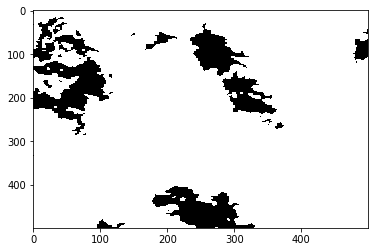
\includegraphics[width=0.35\textwidth]{images/image20} }
	\subfloat[Збільшена маска]{ 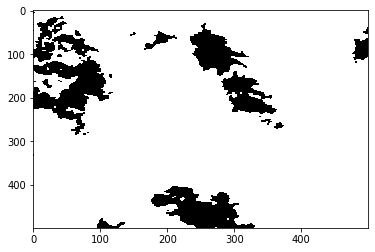
\includegraphics[width=0.35\textwidth]{images/image21} }\\
	\subfloat[Залишки після перетину власної з маскою від COAH]{ 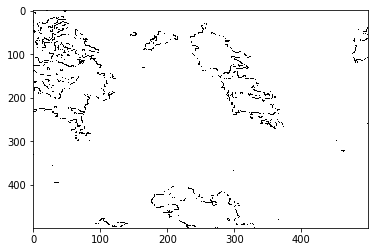
\includegraphics[width=0.35\textwidth]{images/image23} }
	\subfloat[Залишки після перетину власної із уточненою]{ 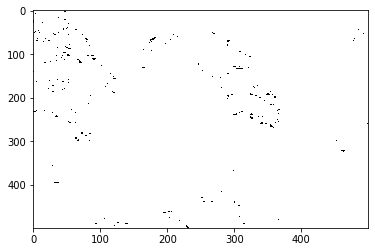
\includegraphics[width=0.35\textwidth]{images/image22} }
	\caption{Приклад уточнення маски хмар \label{fig:cloud-mask-dilation-example} }
\end{figure}

\begin{table}[H]
	\centering
	\caption{Порівняння характеристик масок хмар}
	\label{tab:cloud-mask-comparison}
	\begin{tabular}{|l|r|r|r|}
		\hline
		Метрика                           & COAH          & Еталонна & Уточнена       \\
		\hline
		Частка хмар у масці               & 0,19\%        & 0,22\%   & 0,21\%         \\
		\hline
		Покриття відносно еталонної маски & $\approx 8\%$ & 100\%    & $\approx 95\%$ \\
		\hline
	\end{tabular}
\end{table}

\begin{table}[H]
	\centering
	\caption{Оцінювання точності уточнення маски хмар}
	\label{tab:mask-accuracy}
	\begin{tabular}{|l|r|r|}
		\hline
		Метрика                & COAH    & Уточнена маска \\
		\hline
		Кореляція Пірсона      & 0,89   & 0,93            \\
		\hline
		Кореляція Спірмена     & 0,89   & 0,93            \\
		\hline
		Тау Кендалла           & 0,89   & 0,93            \\
		\hline
		Індекс Жаккара         & 0,83   & 0,89            \\
		\hline
		Евклідова відстань     & 390,61 & 302,98          \\
		\hline
		Мангеттенська відстань & 152579  & 91797          \\
		\hline
	\end{tabular}
\end{table}

Уточнена маска має вищу кореляцію з еталонною %
маскою і менші відстані. Отже, морфологічне розширення краще враховує %
периферію хмар.